\section{Architektur}
\begin{figure}[htp]
      \centering
      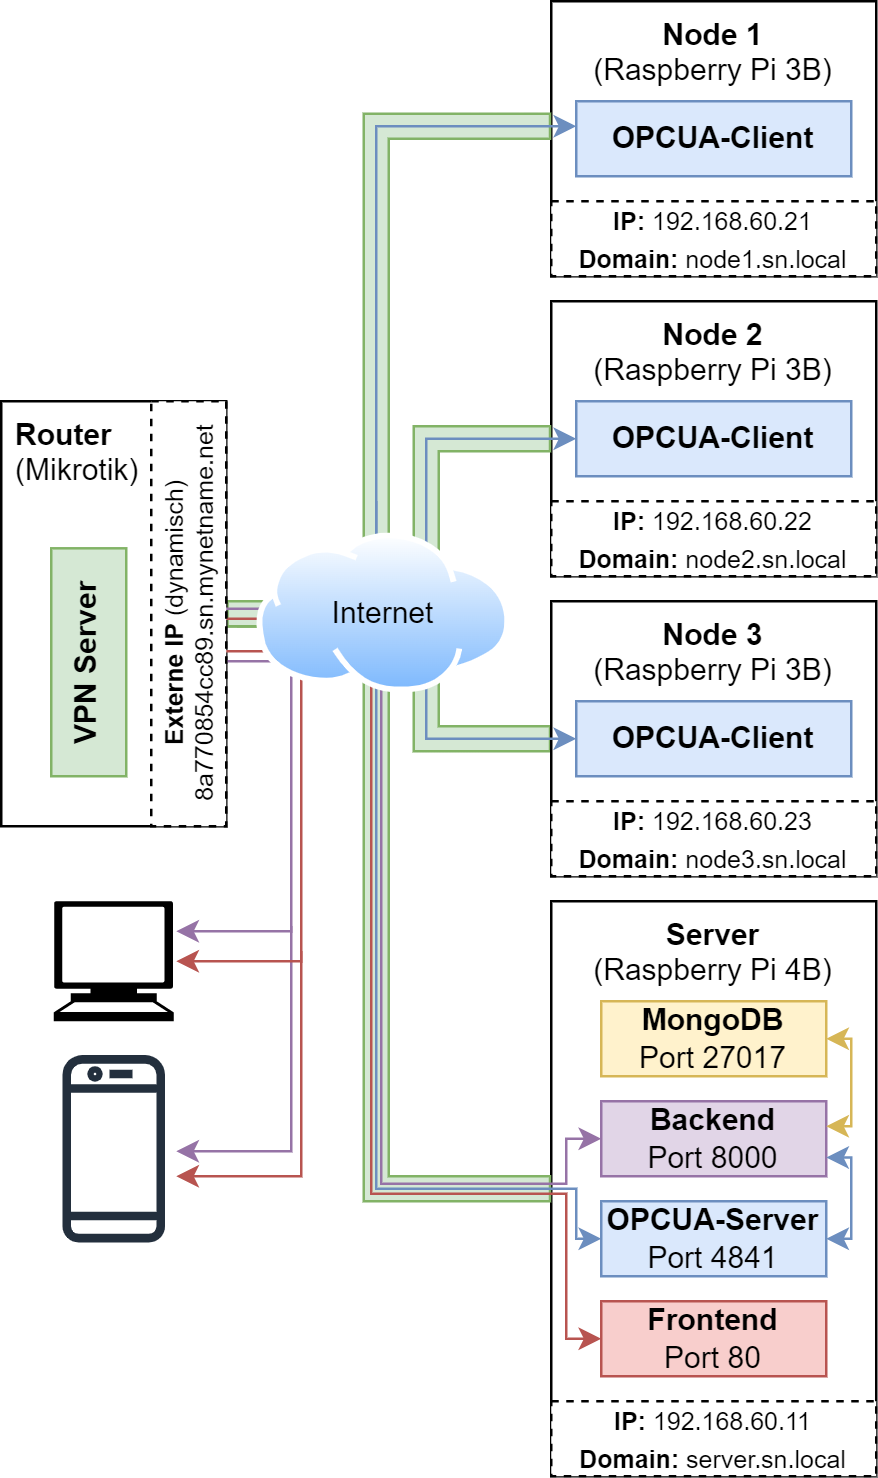
\includegraphics[scale=0.18]{abbildungen/Netzwerkdiagramm.png}
      \caption{Gesamtarchitektur}
      \label{arch}
\end{figure}

\subsection{VPN-Netzwerk}
Um Standortunabhängigkeit zu erreichen, wurde ein VPN Netzwerk auf einem Router aufgesetzt, in welches sich alle Sensorknoten und der Server beim Start automatisch einwählen können.
Die Knoten und der Server erhalten dabei eine feste IP, sowie einen eigene interne Domain. Dies erlaubt eine direkte Kommunikation zwischen den Teilnehmern, über welches auch die OPCUA-Kommunikation abgewickelt wird. 
Der Server stellt zusätzlich eine Web-API, sowie das zugehörige Web-Frontend bereit, welches über diesen aufgerufen werden kann. 


\subsection{Gesamtarchitektur}

Abbildung \ref{arch} zeigt eine Übersicht der Gesamtarchitektur.
Zu sehen ist dabei, dass die Komponenten Frontend, OPCUA-Server, Backend auf dem selben Server laufen.
Dieser Server, sowie die drei OPCUA-Clients, sind dabei über die das VPN verbunden.

Über die externe IP des Routers können Clients auf die Anwendung zugreifen.
